\documentclass[a4paper,12pt]{article}

% Packages
\usepackage[utf8]{inputenc}  % Input encoding
\usepackage[T1]{fontenc}     % Font encoding
\usepackage[english]{babel}  % Language
\usepackage{graphicx}
\usepackage{caption} % Captions
\usepackage{subcaption} % Subcaptions
\usepackage{amsthm}
\usepackage{amsmath}
\newtheorem{theorem}{Theorem}[section]
\newtheorem{definition}{Definition}[section]
\usepackage{amssymb}
\usepackage{xcolor} % Colours
\usepackage{listings} % Code listings
\lstdefinestyle{R}{
    language=R,
    basicstyle=\ttfamily\color{black}, % Monospace font
    %keywordstyle=\color{blue}\bfseries, % Keywords in bold blue
    commentstyle=\color{green!50!black}\itshape, % Comments in italic dark green
    stringstyle=\color{red}, % Strings in red
    numbers=left, % Line numbers on the left
    numberstyle=\tiny\color{gray}, % Style of the line numbers
    stepnumber=1, % Every line is numbered
    numbersep=5pt,
    backgroundcolor=\color{gray!10}, % Light grey background
    frame=single, % Frame around the code
    breaklines=true, % Break long lines
    breakatwhitespace=true,
    showstringspaces=false % Do not show spaces inside strings
}
\usepackage{tikz}
\usetikzlibrary{shapes.geometric, arrows}

% Title information
\title{Homework 2, Computational Statistics}
\author{Alessio Manetti}
\date{\today}  % Automatic compilation date



\begin{document}

% Title page
\maketitle
\tableofcontents  % Automatically generated table of contents

\newpage

\section{Exercise 1}
We assume to have the following coordinates in the two-dimensional space:
\begin{equation*}
    \text{\textbf{s}} = (s_1, s_2) \in \mathbb{R}^2,
\end{equation*}
and the following model:
\begin{equation*}
    Y(\text{\textbf{s}})|W(\text{\textbf{s}}) \overset{\text{iid}}{\sim} GP(W(\text{\textbf{s}}), \tau^2),
\end{equation*}
\begin{equation*}
     W(\text{\textbf{s}}) \sim GP(m(\text{\textbf{s}}), C(||\text{\textbf{s}} - \text{\textbf{s'}}||; \phi, \sigma^2 )),
\end{equation*}
where:
\begin{equation*}
    m(\text{\textbf{s}}) = \beta_0 + \beta_1 s_1,
\end{equation*}
and:
\begin{equation*}
    C(||\text{\textbf{s}} - \text{\textbf{s'}}||; \phi, \sigma^2 ) = \sigma^2 \exp{(-\phi ||\text{\textbf{s}} - \text{\textbf{s'}}||)}.
\end{equation*}
We use the following parameters:
\begin{equation*}
    \tau^2 = 0.5, \ \ \sigma^2 = 0.5, \ \ \phi = \frac{3}{10}, \ \ \beta_0 = 2, \ \ \beta_1 = 0.1.
\end{equation*}

\subsection{}
We want to simulate 100 observations \(\mathbf{y} = \{y_1, ..., y_{100} \}\) from the model at the locations \( \mathbf{D} = \{ \mathbf{s}_1, \dots, \mathbf{s}_{100} \} \), where:
\begin{equation*}
    \mathbf{s_i} \sim U(0,10) \times U(0,10).
\end{equation*}
We start by simulating the coordinates and building the matrix that pairs the x coordinates with the y coordinates:
\begin{lstlisting}[style=R]
n = 100
s1 = runif(n, 0, 10) # x coordinates
s2 = runif(n, 0, 10) # y coordinates

points = cbind(s1, s2) # matrix with the coordinates of the points (x, y)
\end{lstlisting}
We then initialise the parameters:
\begin{lstlisting}[style=R]
tau2 = 0.5
sigma2 = 0.5
phi = 3/10
beta0 = 2
beta1 = 0.1
\end{lstlisting}
and we define the mean and the covariance matrix of \(W(\mathbf{s})\):
\begin{lstlisting}[style=R]
m_s = beta0 + s1 * beta1
distance_matrix = as.matrix(dist(points)) # distance matrix
covariance_matrix = sigma2 * exp(- phi * distance_matrix)
\end{lstlisting}
In order to simulate from a multivariate normal we use the following package:
\begin{lstlisting}[style=R]
library(MASS)
\end{lstlisting}
and we simulate the Gaussian process \(W(\mathbf{s})\):
\begin{lstlisting}[style=R]
W_s = mvrnorm(1, mu = m_s, Sigma = covariance_matrix)
\end{lstlisting}
We can now simulate the Gaussian process \(Y(\mathbf{s})|W(\mathbf{s})\) as:
\begin{equation*}
    Y(\mathbf{s}) = W(\mathbf{s}) + \epsilon, \ \epsilon \sim \mathcal{N}(0, \tau^2)
\end{equation*}
\begin{lstlisting}[style=R]
epsilon = rnorm(n, 0, sqrt(tau2))
Y_s = W_s + epsilon
\end{lstlisting}
For convenience we build the following data set:
\begin{lstlisting}[style=R]
data_sim = data.frame(x = s1, y = s2, W_s = W_s, Y_s = Y_s)
\end{lstlisting}
whose first 3 rows are:
\begin{lstlisting}[style=R]
             x           y       W_s        Y_s
1   7.35633760 5.468326660 2.0160338 1.60076657
2   5.24902455 8.824211084 1.3960101 2.18306186
3   7.62145408 2.089416003 3.6873396 4.30020746
\end{lstlisting}
Below we find the values of \(Y(\mathbf{s})\) and \(W(\mathbf{s})\) in the two-dimensional space:
\begin{figure}[h!]
    \centering
    % First image
    \begin{subfigure}[t]{0.45\textwidth}
        \centering
        
\includegraphics[width=\textwidth]{images/Rplot.png}
        \caption{Simulation of the Gaussian process \(W(\mathbf{s})\).}
        \label{fig:immagine1}
    \end{subfigure}
    \hfill % Flexible space between the images
    % Second image
    \begin{subfigure}[t]{0.45\textwidth}
        \centering
        
\includegraphics[width=\textwidth]{images/Rplot01.png}
        \caption{Simulation of the Gaussian process \(Y(\mathbf{s})\).}
        \label{fig:immagine2}
    \end{subfigure}
    \label{fig:immagini_affiancate}
\end{figure}
\newpage

\subsection{}
We now want to build a scatterplot of the coordinates $(x, y)$, where the points are coloured according to the value of $\mathbf{y}$ following these criteria:
\begin{enumerate}
    \item the first group (first colour) contains the observations with \[\mathbf{y} < \text{25th percentile};\]
    \item the second group (second colour) contains the observations with \[\mathbf{y} \in (\text{25th percentile}, \text{50th percentile}];\]
    \item the third group (third colour) contains the observations with \[\mathbf{y} \in (\text{50th percentile}, \text{75th percentile}];\]
    \item the last group (fourth colour) contains the observations with \[\mathbf{y} > \text{75th percentile}.\]
\end{enumerate}
To do so, we compute the quantiles of the set of values simulated from the Gaussian process \(Y(\mathbf{s})|W(\mathbf{s})\):
\begin{lstlisting}[style=R]
quantiles_y = quantile(data_sim$Y_s, probs = c(0, 0.25, 0.5, 0.75, 1))
\end{lstlisting}
and we add to the data set a column reporting the group each point belongs to:
\begin{lstlisting}[style=R]
data_sim$group = cut(data_sim$Y_s,
                     breaks = quantiles_y,
                     include.lowest = FALSE,
                     include.highest = TRUE,
                     labels = c('0% <= q_i <= 25%', '25% < q_i <= 50%',
                                '50% < q_i <= 75%', '75% < q_i <= 100%'))
\end{lstlisting}
so that the data set now has the following form:
{\scriptsize % Smaller font for this section only
\begin{lstlisting}[style=R]
             x           y       W_s        Y_s             group
1   7.35633760 5.468326660 2.0160338 1.60076657  0% <= q_i <= 25%
2   5.24902455 8.824211084 1.3960101 2.18306186  25% < q_i <= 50%
3   7.62145408 2.089416003 3.6873396 4.30020746 75% < q_i <= 100%
\end{lstlisting}
}
Below we find the graphical representation:
\begin{figure}[h!]
    \centering
    
\includegraphics[width=0.8\textwidth]{images/Rplot02.png}
    \caption{Scatterplot of the coordinates with 4 colours corresponding to the 4 quantile groups.}
    \label{fig:immagine}
\end{figure}

\subsection{}
We now want to choose an arbitrary \(n_{new} \in [10,90]\), and select at random \(n_{new}\) observations out of the \(n\) original observations of \(Y(\mathbf{s})|W(\mathbf{s})\). We collect those observations in the vector \(\mathbf{y_o}\) and the remaining ones in the vector \(\mathbf{y_u}\), and the coordinates corresponding to \(\mathbf{y_o}\) in \(D_o\) and those corresponding to \(\mathbf{y_u}\) in \(D_u\). \\
We want to define appropriate priors for the parameters and write an MCMC algorithm to obtain samples from:
\begin{equation*}
    f(\mathbf{w}, \beta_0, \beta_1, \tau^2, \sigma^2, \phi|\mathbf{y_o}).
\end{equation*}
The corresponding DAG is:
\begin{center}
    \begin{tikzpicture}[node distance=1.5cm]

% Nodes
\node (y_o) [rectangle, draw, align=center] {$\mathbf{y_o}$};
\node (tau) [rectangle, draw, left of=y_o, align=center] {$\tau^2$};
\node (w) [rectangle, draw, right of=y_o, align=center] {$\mathbf{w}$};
\node (sigma) [rectangle, draw, right of=w, align=center] {$\sigma^2$};
\node (phi) [rectangle, draw, below of=sigma, align=center] {$\phi$};
\node (beta) [rectangle, draw, above of=sigma, align=center] {$\boldsymbol{\beta}$};


% Arrows
\draw[->] (tau) -- (y_o);
\draw[->] (sigma) -- (w);
\draw[->] (phi) -- (w);
\draw[->] (beta) -- (w);
\draw[->] (w) -- (y_o);

\end{tikzpicture}
\end{center}


We define the following priors:
\[ \boldsymbol{\beta} \sim \mathcal{N}_2\left(\mathbf{0}, 100 \, \mathbf{I}_2\right), \ \sigma^2 \sim IG(1,1), \ \phi \sim Gamma(1,1),  \]
\[\tau^2 \sim IG(1,1), \ \mathbf{w} \sim \mathcal{N}_{n_{new}}(m(\text{\textbf{s}}), C(||\text{\textbf{s}} - \text{\textbf{s'}}||; \phi, \sigma^2 )),\]
and we initialise the data introduced above:
\begin{lstlisting}[style=R]
n_new = runif(1, 10, 90)
n_new = floor(n_new)
indices <- sample(1:100, n_new)
indices = sort(indices)

y_o = data_sim$Y_s[indices]
D_o = data_sim[indices, c('x', 'y')]

y_u = data_sim$Y_s[-indices]
D_u = data_sim[-indices, c('x', 'y')]
\end{lstlisting}
We set the number of iterations of the MCMC algorithm and we initialise the vectors that will collect the posterior draws of the parameters, setting a starting value for each vector:
\begin{lstlisting}[style=R]
n_iter = 60000

# Starting values
beta0_samples = rep(NA, n_iter)
beta0_samples[1] = 0
beta1_samples = rep(NA, n_iter)
beta1_samples[1] = 0
tau2_samples = rep(NA, n_iter)
tau2_samples[1] = 1
sigma2_samples = rep(NA, n_iter)
sigma2_samples[1] = 1
phi_samples = rep(NA, n_iter)
phi_samples[1] = 0.1
W_samples = matrix(NA, nrow = n_iter, ncol = n_new)
W_samples[1, ] = rep(0,n_new)
\end{lstlisting}
We select the values of the x coordinates (\(s_1\)) corresponding to the selected observations and we build the new distance matrix for those observations:
\begin{lstlisting}[style=R]
D_o_x = data_sim[indices, c('x')]
distance_matrix_o = as.matrix(dist(D_o))
\end{lstlisting}
and we also build the new design matrix \(\mathbf{X}\):
\begin{lstlisting}[style=R]
ones = rep(1, n_new)
X = cbind(ones, D_o_x)
\end{lstlisting}
We are now ready to start the iterations of the MCMC algorithm:
\begin{lstlisting}[style=R]
for (i in 2:n_iter)
{
    # ...
}
\end{lstlisting}
The first step of the MCMC algorithm is the update of the posterior value \(\boldsymbol{\beta}|\mathbf{w}\). \\
We know from the theory that:
\begin{align*}
    \boldsymbol{\beta}|\mathbf{w} &\sim \mathcal{N}_2(M_2,V_2), \\
    V_2 &= \left( \mathbf{X}^T C^{-1} \mathbf{X} + \begin{pmatrix}
\frac{1}{100} & 0 \\
0 & \frac{1}{100}
\end{pmatrix} \right)^{-1} \\
    M_2 &= V_2 \left( \mathbf{X}^T C^{-1} \mathbf{w} \right)
\end{align*}
We compute the covariance matrix \(C_o(\cdot)\) corresponding to the selected observations and we invert it:
\begin{lstlisting}[style=R]
C_o = sigma2_samples[i-1] * exp(- phi_samples[i-1] * distance_matrix_o)
inv_C_o = solve(C_o)
\end{lstlisting}
and we sample \(\boldsymbol{\beta}\):
\begin{lstlisting}[style=R]
## Step (1): update of beta
# Vp
Vp = solve(t(X) %*% inv_C_o %*% X + diag_matrix)

# Mp
Mp = Vp %*% (t(X) %*% inv_C_o %*% W_samples[i-1,])

# Sample beta
beta = mvrnorm(1, Mp, Vp)
beta0_samples[i] = beta[1]
beta1_samples[i] = beta[2]
\end{lstlisting}
The second step is the update of the posterior value \(\sigma^2|\mathbf{w}\). \\
Using the kernel method, we find its posterior distribution:
\begin{align*}
    f(\sigma^2|\mathbf{w}) &\propto f(\mathbf{w}|\sigma^2)f(\sigma^2) \\
    &\propto (\sigma^2)^{-\left( \frac{n_{new}}{2} + a + 1 \right)} \exp{\left\{ - \frac{\left[ \frac{(\mathbf{w} - \mathbf{X} \boldsymbol{\beta})^T C^{-1} (\mathbf{w} - \mathbf{X} \boldsymbol{\beta})}{2} + b \right]}{\sigma^2} \right\}},
\end{align*}
that is:
\begin{equation*}
    \sigma^2|\mathbf{w} \sim IG\left(\frac{n_{new}}{2} + a, \frac{(\mathbf{w} - \mathbf{X} \boldsymbol{\beta})^T C^{-1} (\mathbf{w} - \mathbf{X} \boldsymbol{\beta})}{2} + b \right),
\end{equation*}
where in our case \(a = b = 1\).\\
We therefore sample \(\sigma^2\):
\begin{lstlisting}[style=R]
## Step (2): update of sigma2
a_sigma2 = n_new/2 + 1
quad_form = t(W_samples[i-1,] - X %*% beta) %*% inv_C_o %*% (W_samples[i-1,] - X %*% beta)
b_sigma2 = quad_form/2 + 1

# Sample sigma2
sigma2_samples[i] = 1 / rgamma(1, a_sigma2, b_sigma2)
\end{lstlisting}
The third step is the update of the posterior value \(\tau^2|\mathbf{y_o}\). \\
Using the kernel method, we find its posterior distribution:
\begin{align*}
    f(\tau^2|\mathbf{y_o}) &\propto f(\mathbf{y_o}|\tau^2)f(\tau^2) \\
    &\propto (\tau^2)^{-\left( \frac{n_{new}}{2} + a + 1 \right)} \exp{\left\{ - \frac{\left[ \frac{(\mathbf{y_o - \mathbf{w}})^T (\mathbf{y_o - \mathbf{w}})}{2} + b \right]}{\tau^2} \right\}},
\end{align*}
that is:
\begin{equation*}
    \tau^2|\mathbf{y_o} \sim IG\left(\frac{n_{new}}{2} + a, \frac{(\mathbf{y_o} - \mathbf{w})^T (\mathbf{y_o} - \mathbf{w})}{2} + b \right),
\end{equation*}
where in our case \(a = b = 1\).\\
We therefore sample \(\tau^2\):
\begin{lstlisting}[style=R]
## Step (3): update of tau2
a_tau2 = n_new/2 + 1
b_tau2 = 0.5 * t(y_o - W_samples[i-1,]) %*% (y_o - W_samples[i-1,]) + 1

# Sample tau2
tau2_samples[i] = 1 / rgamma(1, a_tau2, b_tau2)
\end{lstlisting}
The fourth step is the update of the posterior value \(\phi|\mathbf{w}\). \\
Since the form of that distribution is hard to obtain in closed form, we use the Metropolis algorithm. \\
A new value for the parameter \(\phi\) is proposed; the proposed value, denoted by \(\phi_{prop}\), is generated from a normal distribution centred on the value of \(\phi\) at the \(i\)-th iteration, with adaptive standard deviation (initialised at the value 0.1). \\
After proposing the new value, we check that \(\phi_{prop}\) lies between two bounds computed from the spatial distances between the points.
If the proposed value does not satisfy this condition, it is discarded:
\begin{lstlisting}[style=R]
## Step (4): update of phi (Metropolis)
phi_prop = rnorm(1, phi_samples[i-1], sd_proposal)
if (phi_prop >= 3/max(dist(points)) && phi_prop <= 3/min(dist(points)))
{
    # ...
}
\end{lstlisting}
Next, we compute the logarithm of the ratio between the likelihood and the log-prior of the parameter \(\phi\), at the current and at the proposed value. The covariance matrix is rebuilt at the value of \(\phi\) it refers to, otherwise the ratio would depend on the prior alone. This log-ratio is given by:
\begin{lstlisting}[style=R]
C_prop = sigma2_samples[i] * exp(- phi_prop * distance_matrix_o)
C_curr = sigma2_samples[i] * exp(- phi_samples[i-1] * distance_matrix_o)

log_ratio = log_fc_phi(phi_prop, W_samples[i-1,], beta, sigma2_samples[i], X, C_prop) - log_fc_phi(phi_samples[i-1], W_samples[i-1,], beta, sigma2_samples[i], X, C_curr)
\end{lstlisting}
The function \texttt{log\_fc\_phi()} computes the logarithm of the likelihood and the log-prior of \texttt{phi}. The likelihood is based on the determinant of the covariance matrix \(C\) and on the residual between the observations and the predictions, while the log-prior assumes a Gamma distribution for \(\phi\). If the log-ratio is positive, the proposal is accepted with higher probability:
\begin{lstlisting}[style=R]
log_fc_phi = function(phi, w, beta, sigma2, X, C)
{
  # Determinant
  det_C = determinant(C, logarithm = TRUE)$modulus  # log-determinant

  det_C = abs(det_C)  # abs is used in case the determinant is negative

  # Log-likelihood
  res = w - X %*% beta
  log_likelihood = -0.5 * (det_C + t(res) %*% solve(C) %*% res)

  # Log-prior of phi, Gamma distributed
  log_prior = dgamma(phi, 1, 1, log = TRUE)

  return(log_likelihood + log_prior)
}
\end{lstlisting}
The acceptance probability (initially set to 0) is given by:
\begin{lstlisting}[style=R]
min(exp(log_ratio), 1)
\end{lstlisting}
If a uniform random number between 0 and 1 is smaller than the acceptance probability, the proposed value \(\phi_{prop}\) is accepted as the new value of \(\phi\):
\begin{lstlisting}[style=R]
if (runif(1, 0, 1) < exp(log_ratio))
{
    phi = phi_prop
}
\end{lstlisting}
Otherwise, the value of \(\phi\) is left unchanged. Every 50 iterations, the standard deviation of the proposal is adapted so as to keep the acceptance rate of the proposals close to the target value 0.234. This adaptation is carried out as follows:
\begin{lstlisting}[style=R]
nbatch = 50
A = 100
B = 1000
alpha_target = 0.234

if (i%%nbatch == 0)
{
    alpha_phi = alpha_phi / nbatch
    sd_proposal = exp(log(sd_proposal) + A / (B + i) * (alpha_phi - alpha_target))
    alpha_phi = 0
}
\end{lstlisting}
Finally, the updated value of \texttt{phi} is stored as:
\begin{lstlisting}[style=R]
phi_samples[i] = phi
\end{lstlisting}
The fifth step is the update of the posterior value \(\mathbf{w}|\mathbf{y_o}\). \\
Using the kernel method, we find its posterior distribution:
\begin{align*}
    f(\mathbf{w}|\mathbf{y_o}) &\propto f(\mathbf{y_o}|\mathbf{w})f(\mathbf{w}) \\
    &\propto \exp{\left\{ - \frac{\mathbf{w}^T\mathbf{Q}\mathbf{w}}{2} + \mathbf{b}^T \mathbf{w}\right\}},
\end{align*}
where:
\begin{align*}
    \mathbf{Q} &= \frac{\mathbf{I}}{\tau^2} + C^{-1}, \\
    \mathbf{b} &= \frac{\mathbf{y_o}}{\tau^2} + C^{-1} \mathbf{X} \mathbf{\beta},
\end{align*}
that is:
\begin{equation*}
    \mathbf{w}|\mathbf{y_o} \sim \mathcal{N}_{n_{new}}(\mathbf{Q}^{-1}\mathbf{b}, \mathbf{Q}^{-1}).
\end{equation*}
We therefore sample \(\mathbf{w}\):
\begin{lstlisting}[style=R]
# Step (5): update of W
  Q = inv_C_o + diag(1 / tau2_samples[i], n_new)
  b = inv_C_o %*% X %*% beta + y_o / tau2_samples[i]
  muW_post = solve(Q) %*% b
  sigmaW_post = solve(Q)

  # Sample W
  W_samples[i,] = mvtnorm::rmvnorm(1, as.vector(muW_post), sigmaW_post)
\end{lstlisting}
We now look at the trace plots of the samples obtained for each parameter, running 60000 iterations and applying a burn-in of the first 20000 iterations: \\
\begin{figure}[h!]
    \centering
    % First row
    
\includegraphics[width=0.42\textwidth]{images/Rplot03.png}
    
\includegraphics[width=0.42\textwidth]{images/Rplot04.png} \\\vspace{0.5cm}
    % Second row
    
\includegraphics[width=0.42\textwidth]{images/Rplot05.png}
    
\includegraphics[width=0.42\textwidth]{images/Rplot06.png} \\\vspace{0.5cm}
    % Last image
    
\includegraphics[width=0.42\textwidth]{images/Rplot07.png}
    \caption{MCMC estimates.}
    \label{fig:organized_images}
\end{figure}
\\
We obtained the following results:
\begin{table}[ht]
\centering
\begin{tabular}{lc}
\hline
\textbf{Parameter} & \textbf{Effective samples} \\
\hline
$\beta_0$ & 38078.08 \\
$\beta_1$ & 37902.33 \\
$\tau^2$  & 13535.94 \\
$\sigma^2$ & 27174.99 \\
$\phi$    & 1553.615 \\
\hline
\end{tabular}
%\caption{Effective sample size of the MCMC estimates}
\label{tab:effective_samples}
\end{table}

\subsection{}
We now want to obtain samples from the posterior of:
\begin{equation*}
    \epsilon(\boldsymbol{s}) = Y(\boldsymbol{s}) - (\beta_0 + \beta_1 s_1), \quad \boldsymbol{s} \in D_o.
\end{equation*}
First, we create the matrix that will contain the posterior draws of \(\epsilon(\boldsymbol{s})\) at each observed \(\boldsymbol{s}\):
\begin{lstlisting}[style=R]
epsilon_samples = matrix(NA, nrow = n_iter - burn_in, ncol = n_new)
\end{lstlisting}
Next, we iterate over all the posterior draws obtained in the previous points, that is those after the burn-in:
\begin{lstlisting}[style=R]
for (i in (burn_in + 1) : n_iter) {
  # ...
}
\end{lstlisting}
Inside the loop we build, using the samples obtained before, the value of \(\epsilon(\boldsymbol{s})\):
\begin{lstlisting}[style=R]
m_post = beta0_samples[i] + beta1_samples[i] * D_o$x
epsilon_samples[i - burn_in, ] = y_o - m_post
\end{lstlisting}
We compute the posterior mean and we add it to the data set:
\begin{lstlisting}[style=R]
epsilon_mean = apply(epsilon_samples, 2, mean)
D_o$epsilon_mean = epsilon_mean
\end{lstlisting}
Below we find the spatial distribution of the mean:
\begin{figure}[h!]
    \centering
    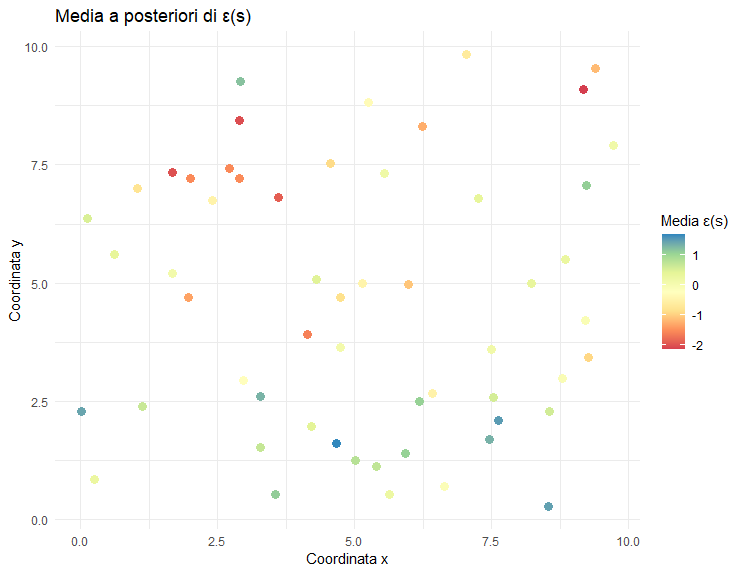
\includegraphics[width=0.8\textwidth]{images/Rplot15.png}
    \caption{Spatial distribution of the mean of \(\epsilon(\boldsymbol{s})\).}
    \label{fig:immagine}
\end{figure}
\newpage

\subsection{}
We now want to obtain samples from the posterior of:
\begin{equation*}
    f(y(\boldsymbol{s}) | \boldsymbol{y}_o), \quad \boldsymbol{s} \in D_u^* \subseteq D_u.
\end{equation*}
We build the set \(D_u^*\) by choosing 20 coordinates among the unobserved ones:
\begin{lstlisting}[style=R]
n_Du_star = 20
indices_Du_star = sample(1:nrow(D_u), n_Du_star)
D_u_star = D_u[indices_Du_star, ]
true_values = y_u[indices_Du_star]
\end{lstlisting}
and we build the distance matrix based on those coordinates:
\begin{lstlisting}[style=R]
distance_matrix_u = as.matrix(dist(D_u_star))
\end{lstlisting}
Next, we initialise the matrix that will contain the posterior draws of \(f(\cdot)\):
\begin{lstlisting}[style=R]
y_s_samples = matrix(NA, nrow = n_iter - burn_in, ncol = n_Du_star)
\end{lstlisting}
We iterate again over the number of draws after the burn-in:
\begin{lstlisting}[style=R]
for (j in (burn_in + 1) : n_iter) {
  # ...
}
\end{lstlisting}
Inside the loop we compute the function \(m(\boldsymbol{s})\) using the posterior draws and the abscissae of the coordinates contained in \(D_u^*\):
\begin{lstlisting}[style=R]
m_s = beta0_samples[j] + D_u_star$x * beta1_samples[j]
\end{lstlisting}
and we generate samples from \(Y(\boldsymbol{s})\) exactly as in the first point:
\begin{lstlisting}[style=R]
covariance_matrix = sigma2_samples[j] * exp(- phi_samples[j] * distance_matrix_u)
W_s = mvrnorm(1, mu = m_s, Sigma = covariance_matrix)
epsilon = rnorm(n_Du_star, 0, sqrt(tau2_samples[j]))
y_s_samples[j - burn_in, ] = W_s + epsilon
\end{lstlisting}
We compute 95\% credible intervals:
\begin{lstlisting}[style=R]
conf_intervals = matrix(NA,n_Du_star,2)

for (i in 1:n_Du_star) {
  conf_intervals[i,1] = quantile(y_s_samples[,i], 0.025)
  conf_intervals[i,2] = quantile(y_s_samples[,i], 0.975)
}
\end{lstlisting}
and we check whether each of the \textit{true values} computed above lies inside the corresponding credible interval:
\begin{lstlisting}[style=R]
is_inside = sapply(1:n_Du_star, function(i) {
  true_values[i] >= conf_intervals[i, 1] && true_values[i] <= conf_intervals[i, 2]
})
\end{lstlisting}
We obtain that all the \textit{true values} lie inside the credible interval:
\begin{figure}[h!]
    \centering
    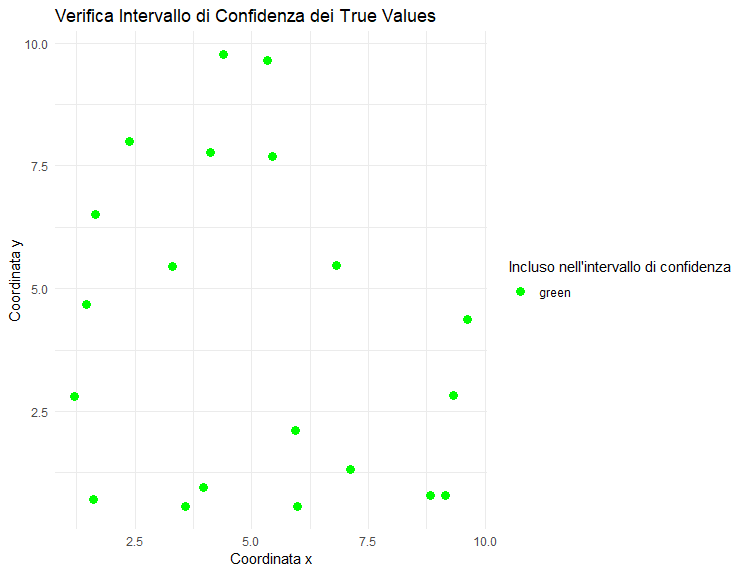
\includegraphics[width=0.8\textwidth]{images/Rplot16.png}
    \caption{95\% credible intervals and true values.}
    \label{fig:immagine}
\end{figure}


\newpage

\section{Exercise 2}
We have a mixture model:
\begin{equation*}
    Y_i|z_i \sim P(\lambda_{z_i}),
\end{equation*}
with latent variable \(\mathbf{z}\) distributed as:
\begin{equation*}
    \mathbb{P}(z_i = k) = \pi_k.
\end{equation*}
where \(i = 1,...,200\), \(z_i \in \{1,2,3\}\), \(\pi_k = \frac{1}{3}, k = 1,2,3\), and:
\begin{equation*}
    \lambda_1 = 1, \ \lambda_2 = 10, \ \lambda_3 = 25.
\end{equation*}

\subsection{}
We want to simulate from the model and represent the data graphically. \\
We initialise the data and simulate the variables \(z_i\) and \(Y_i, \ i = 1,...,200\):
\begin{lstlisting}[style=R]
n = 200
Y = rep(NA, n)
lambda_vec = c(1, 10, 25)
z = rep(NA, n)

for (i in 1:n)
{
  sim = sample(1:3, 1)
  z[i] = sim
  Y[i] = rpois(1, lambda_vec[sim])
}
\end{lstlisting}
Next, we display the observations of \(\mathbf{Y}\), split according to the group they belong to, and their density:
\begin{figure}[h!]
    \centering
    % First image
    \begin{subfigure}[b]{0.48\textwidth}
        \centering
        
\includegraphics[width=\textwidth]{images/Rplot08.png}
        \caption{Observations obtained by simulating \(\mathbf{Y}\).}
        \label{fig:image1}
    \end{subfigure}
    \hfill
    % Second image
    \begin{subfigure}[b]{0.48\textwidth}
        \centering
        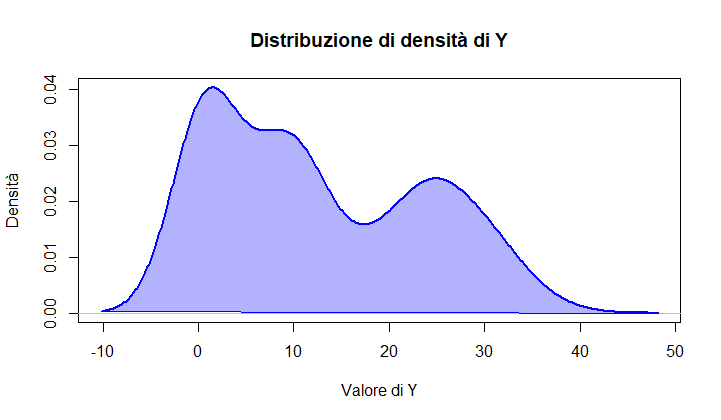
\includegraphics[width=\textwidth]{images/Rplot09.png}
        \caption{Empirical density of \(\mathbf{Y}\).}
        \label{fig:image2}
    \end{subfigure}
    \label{fig:side_by_side}
\end{figure}
\newpage
It is also possible to visualise the overlaid distributions of the points and the combination of boxplots and distributions for each group:
\begin{figure}[h!]
    \centering
    % First image
    \begin{subfigure}[b]{0.48\textwidth}
        \centering
        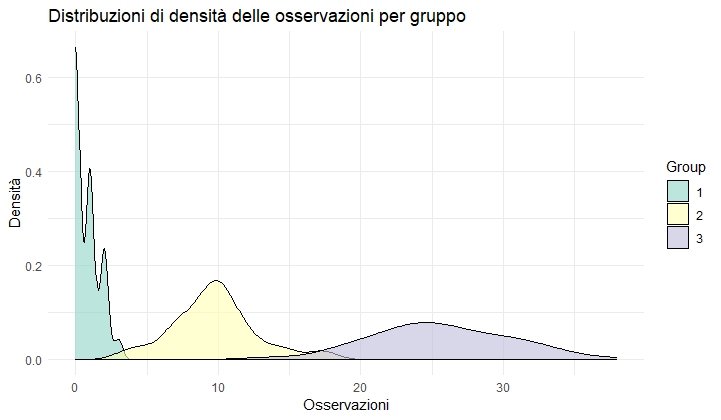
\includegraphics[width=\textwidth]{images/Rplot10.png}
        \caption{Distributions of the observations obtained by simulating \(\mathbf{Y}\), split by group.}
        \label{fig:image1}
    \end{subfigure}
    \hfill
    % Second image
    \begin{subfigure}[b]{0.48\textwidth}
        \centering
        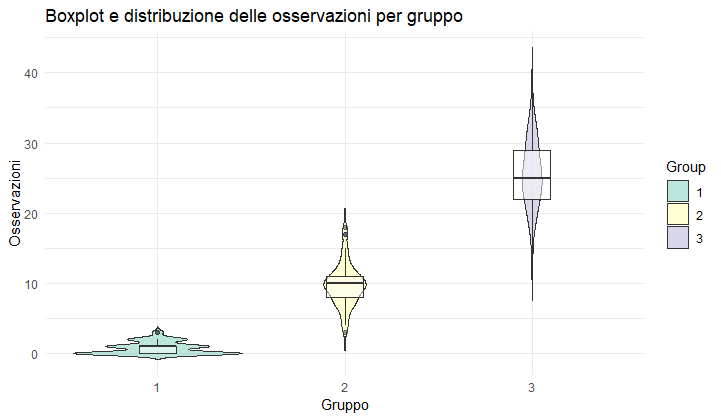
\includegraphics[width=\textwidth]{images/Rplot11.png}
        \caption{Boxplots and distributions of the observations obtained by simulating \(\mathbf{Y}\), split by group.}
        \label{fig:image2}
    \end{subfigure}
    \label{fig:side_by_side}
\end{figure}

\subsection{}
We now want to implement an MCMC method to obtain posterior estimates of:
\begin{equation*}
    f(\lambda_1,\lambda_2,\lambda_3,\pi_1,\pi_2,\pi_3,z_1,...,z_n|\mathbf{y}).
\end{equation*}
We will use the following priors:
\begin{equation*}
    \lambda_k \sim \text{Gamma}(a_{prior},b_{prior}), \ \  \boldsymbol{\pi} \sim \text{Dir}(\boldsymbol{\alpha_{prior}}), \ \ z_i|\boldsymbol{\pi} \sim \text{Discrete}(\boldsymbol{\pi}),
\end{equation*}
for \(k = 1,2,3\), and \(i = 1,...,200\). \\
First, we initialise the parameters:
\begin{lstlisting}[style=R]
n_iter = 10000
k = 3
a_gamma_prior = 1
b_gamma_prior = 1
alpha_prior = c(1,1,1)
\end{lstlisting}
and the matrices that will contain each update of the parameters:
\begin{lstlisting}[style=R]
lambda_samples = matrix(NA, nrow = n_iter, ncol = k)
pi_samples = matrix(NA, nrow=n_iter, ncol=k)
zi_samples = matrix(NA, nrow=n_iter, ncol=n)
\end{lstlisting}
Next, we define the starting values for the MCMC method:
\begin{lstlisting}[style=R]
lambda = rep(mean(Y), k)
pi = rep(1/k, k)
z = sample(1:k, n, replace = TRUE)
\end{lstlisting}
and we run the loop for the chosen number of iterations:
\begin{lstlisting}[style=R]
for (i in 1:n_iter)
{
    # ...
}
\end{lstlisting}
The first step of the MCMC algorithm is the update of the posterior value \(\lambda_k|\mathbf{y},\mathbf{z}\). \\
Using the kernel method, we find its posterior distribution:
\begin{align*}
    f(\lambda_k|\mathbf{y},\mathbf{z}) &\propto f(\mathbf{y}|\lambda_k,\mathbf{z}) f(\lambda_k) \\
    &\propto \lambda_k^{\sum_{i: z_i = k} y_i + a_{prior} - 1} e^{-(n_k + b_{prior}) \lambda_k},
\end{align*}
that is:
\begin{equation*}
    \lambda_k|\mathbf{y},\mathbf{z} \sim \text{Gamma}\left(a_{prior} + \sum_{i: z_i = k} y_i, b_{prior} + n_k \right),
\end{equation*}
where in our case \(a_{prior} = b_{prior} = 1\).\\
We therefore sample \(\lambda_k\):
\begin{lstlisting}[style=R]
## Step (1): update of lambda_k
for (j in 1:k)
{
  Y_j = Y[z == j]
  lambda[j] = rgamma(1, a_gamma_prior + sum(Y_j), b_gamma_prior + length(Y_j))
}

lambda_samples[i,] = lambda
\end{lstlisting}
The second step of the MCMC algorithm is the update of the posterior value \(\boldsymbol{\pi}|\mathbf{z},\mathbf{y}\). \\
Using the kernel method, we find its posterior distribution:
\begin{align*}
    f(\boldsymbol{\pi}|\mathbf{z},\mathbf{y}) &\propto f(\mathbf{y}|\boldsymbol{\pi}, \boldsymbol{z}) f(\boldsymbol{\pi}) \\
    &\propto \prod_{k = 1}^K \pi_k^{\alpha_k + n_k - 1},
\end{align*}
that is:
\begin{equation*}
    \pi_k|\mathbf{z},\mathbf{y} \sim \text{Dir}(\alpha_k + n_k),
\end{equation*}
for \(k = 1,...,K\), with \(K = 3\). \\
We therefore sample \(\boldsymbol{\pi}\):
\begin{lstlisting}[style=R]
## Step (2): update of pi_k
n_k = table(factor(z, levels = 1:k))
pi = rdirichlet(1, alpha_prior + n_k)
pi_samples[i,] = pi
\end{lstlisting}
The third step of the MCMC algorithm is the update of the posterior value \(z_i|y_i,\boldsymbol{\lambda},\boldsymbol{\pi}\). \\
Using the kernel method, we find its posterior distribution:
\begin{align*}
    f(z_i|y_i,\boldsymbol{\lambda},\boldsymbol{\pi}) &\propto f(y_i|z_i,\boldsymbol{\pi}) f(z_i|\boldsymbol{\pi}) \\
    &\propto \pi_k \lambda_k^{y_i} e^{-\lambda_k},
\end{align*}
that is:
\begin{equation*}
    z_i|y_i,\boldsymbol{\lambda},\boldsymbol{\pi} \sim \pi_k P(\lambda_k),
\end{equation*}
where \(k\) is the group \(z_i\) belongs to. \\
When sampling \(z_i\) we compute the probability of \(z_i\) belonging to each group and only afterwards we sample:
\begin{lstlisting}[style=R]
## Step (3): update of z_i
for (j in 1:n)
{
    log_prob_non_norm = c(0,0,0)
    log_prob_non_norm[1] = log(pi[1]) + dpois(Y[j], lambda[1], log = TRUE)
    log_prob_non_norm[2] = log(pi[2]) + dpois(Y[j], lambda[2], log = TRUE)
    log_prob_non_norm[3] = log(pi[3]) + dpois(Y[j], lambda[3], log = TRUE)
    c = max(log_prob_non_norm)
    prob = exp(log_prob_non_norm - (c + log(sum(exp(log_prob_non_norm - c)))))
    z[j] = sample(1:k, 1, prob = prob)
}
zi_samples[i,] = z
\end{lstlisting}
We can now show the plots of the results obtained:

\begin{figure}[h]
  \centering
  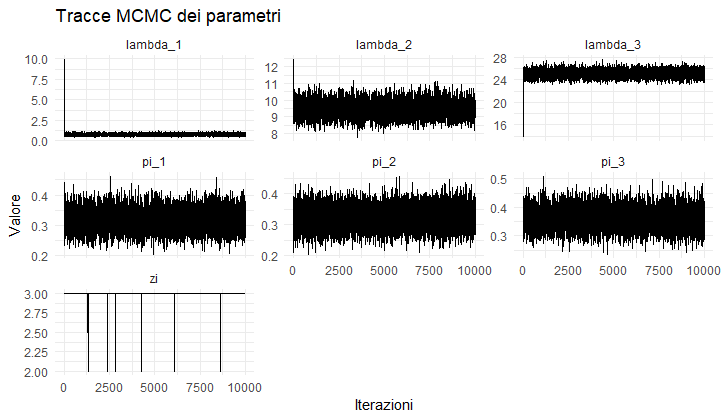
\includegraphics[width=0.95\textwidth]{images/Rplot12.png}
  \caption{Plots of the results obtained}
  \label{fig:esempio_immagine}
\end{figure}






\end{document}
